\documentclass{article}

\usepackage[english]{babel}
\usepackage{tikz}
\usetikzlibrary{patterns,hobby,snakes}
\usepackage{pgfplots}
\pgfplotsset{compat=1.6}
\usepgfplotslibrary{fillbetween}
\usepackage{tabularx,booktabs}
\usepackage[utf8]{inputenc}
\usepackage[T1]{fontenc}
\usepackage{graphicx}
\usepackage{amsfonts}

\begin{document}

%\begin{frame}
%\frametitle{Monte Carlo in path space: the shooting algorithm}
%\begin{block}
%\begin{itemize}
%    \item Start with an initial biased reactive trajectory
%\end{itemize}
%\end{block}
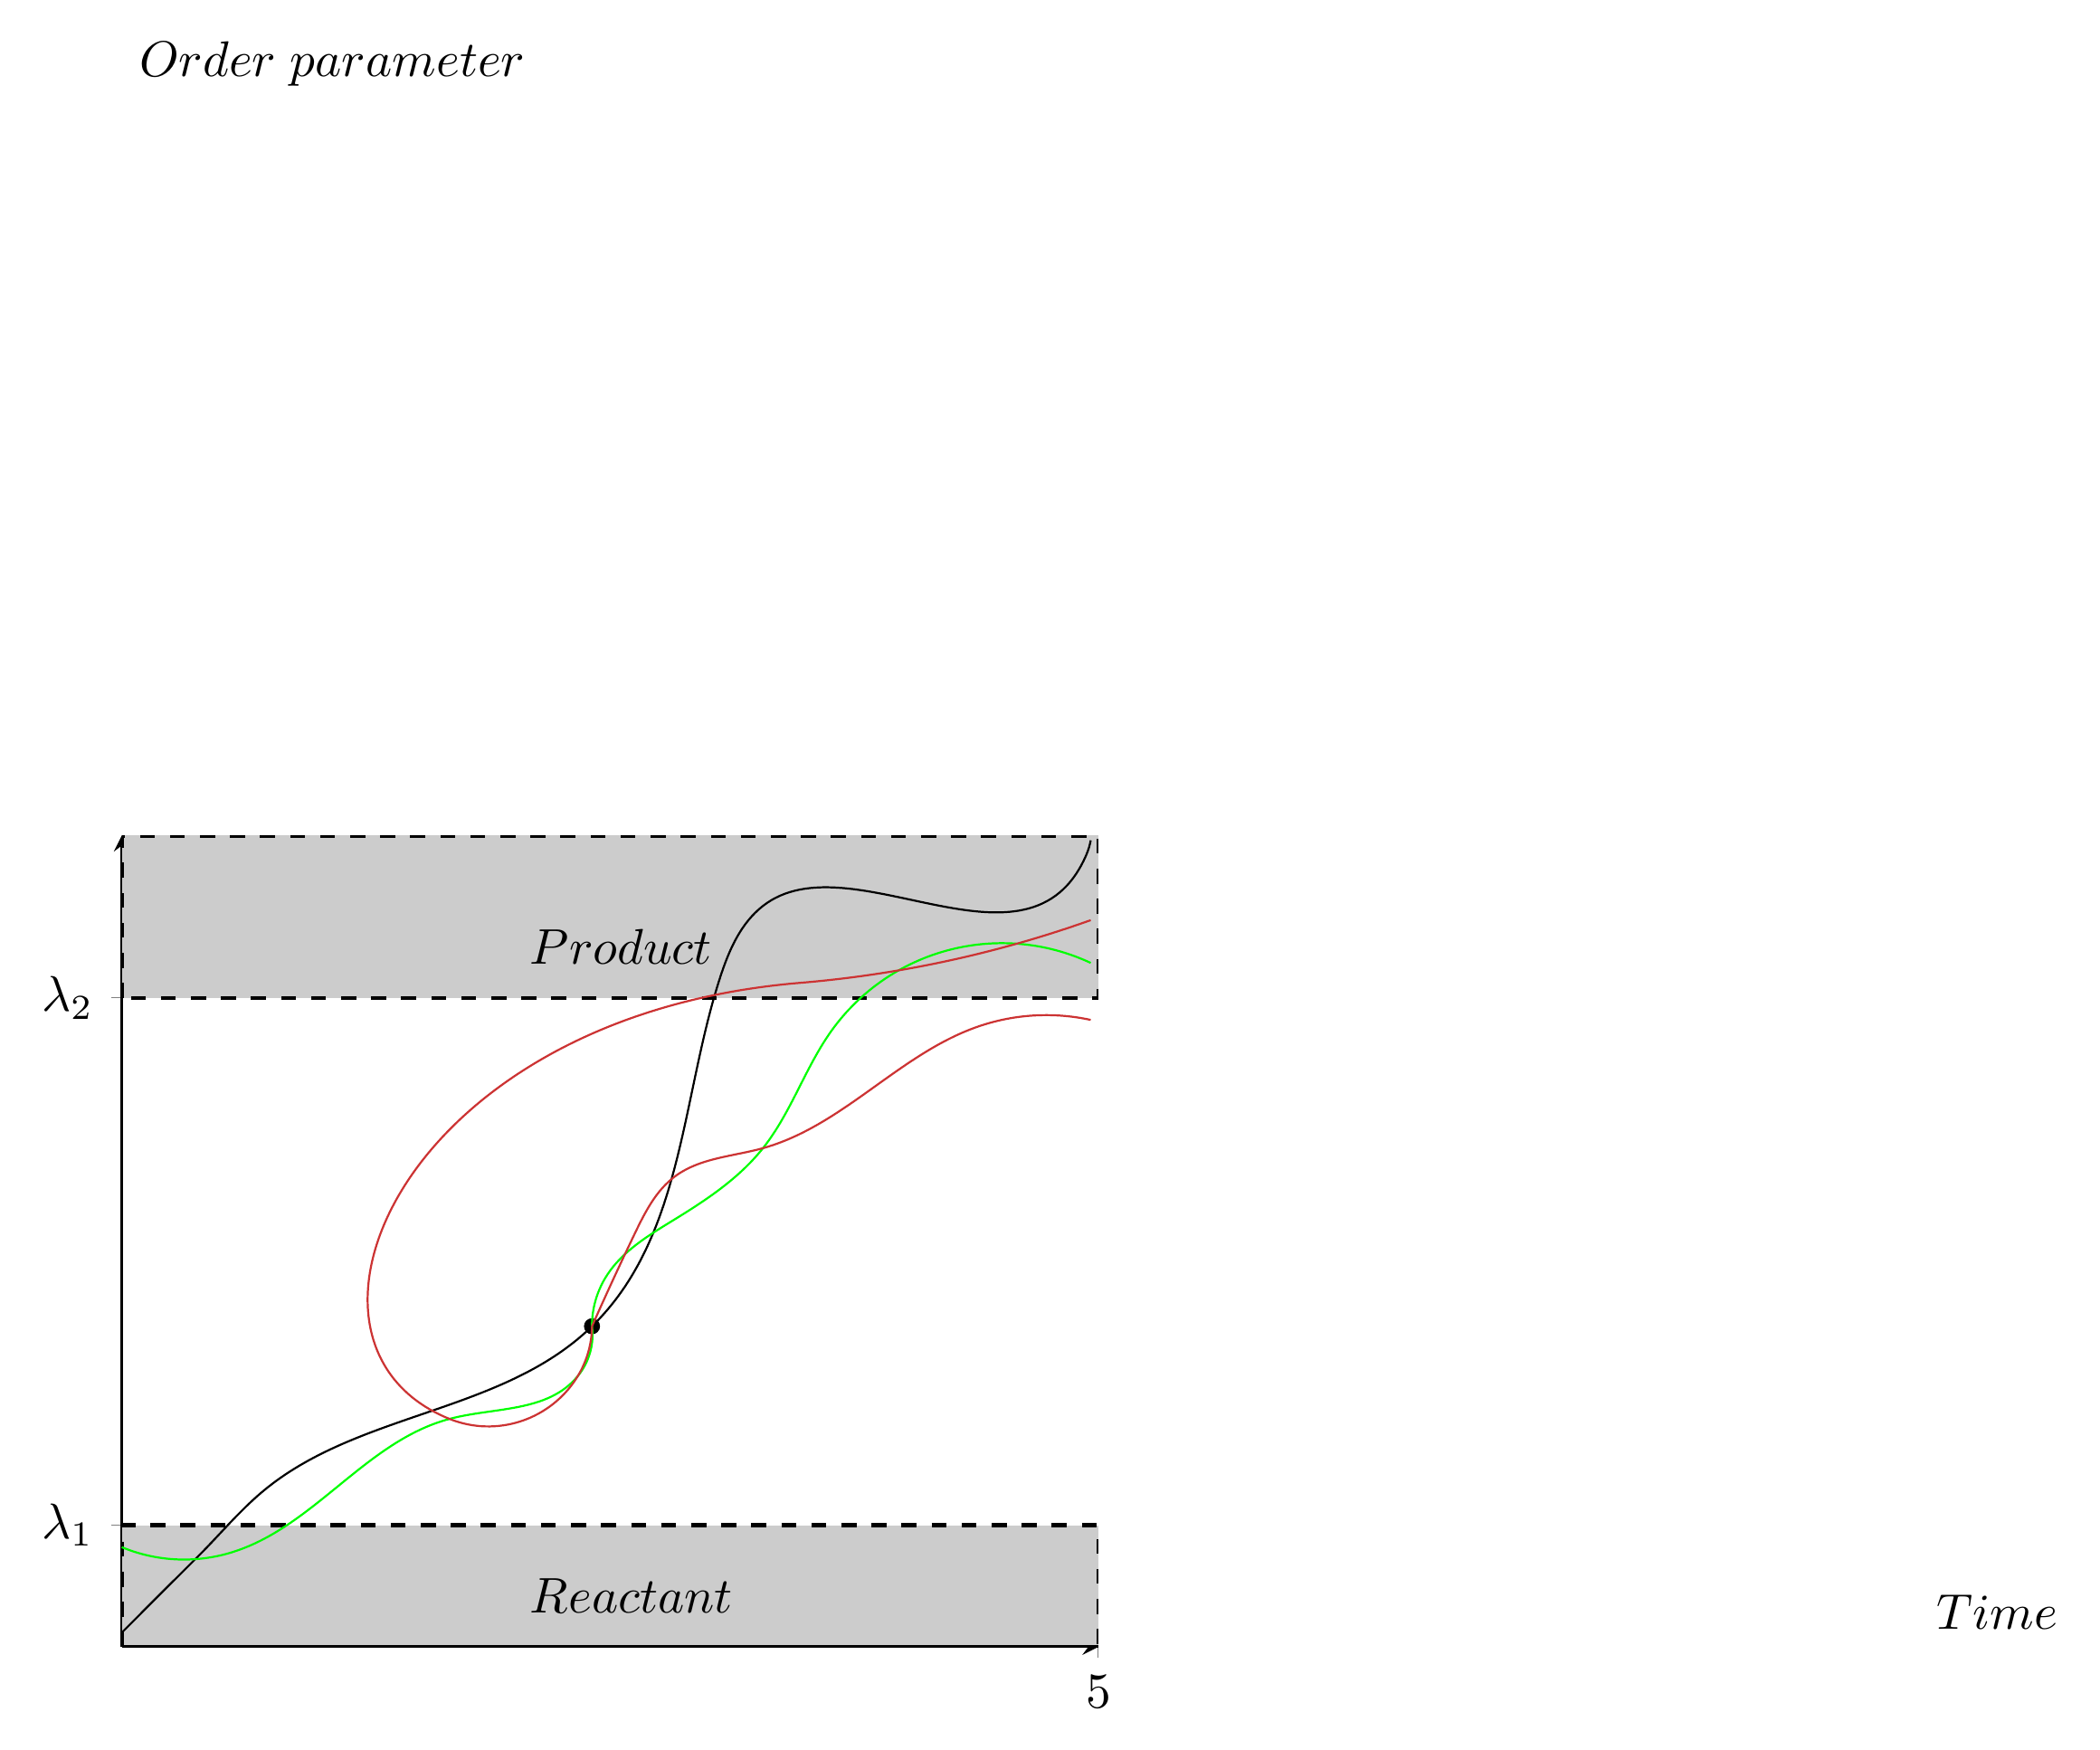
\begin{tikzpicture}[scale=2.0]
 \begin{axis}[
        xmin=0.0,xmax=5.0,
        ymin=0,ymax=5.0,
        xtick={0.0, 5.0},
        %xticklabels={$v_1$,$v_2$},
        ytick={0.75,4.0},
        yticklabels={$\lambda_1$,$\lambda_2$},
        xlabel={$Time$},  
        ylabel={$Order\;parameter$},
        every axis x label/.style={
    at={(ticklabel* cs:5.05)},
    anchor=west,
},
every axis y label/.style={
    at={(ticklabel* cs:5.05)},
    anchor=south,
},
        axis lines=middle] 
    \draw [fill=gray!40!white,thick,dashed] (axis cs:0,0) rectangle (axis cs:5.0,0.75);
    \draw [fill=gray!40!white,thick,dashed] (axis cs:0,4.0) rectangle (axis cs:5.0,5.0);
    \addplot+[black,thick,domain=0:5,no marks] {0};
    %
    \node  at (axis cs:2.0,4.1)    [anchor=south west] {$Product$};
    \node  at (axis cs:2.0,0.1)    [anchor=south west] {$Reactant$};
    \end{axis}
\draw [thick] (0.0 ,0.1)  to [ curve through ={(0.5, 0.6) . . (0.55, 0.65)  . . (1.0,1.1) . . (3.3, 2.25) . . (4.2, 4.7) . . (4.5,5.2) . . (6.77, 5.56)  }] (6.8,5.66) ;% curve 
\filldraw (3.3,2.25) circle[radius=1.5pt];
\draw [green,thick] (3.3 ,2.25) to [ curve through ={(3.4,2.6)  . . (3.88, 3.00) . . (4.5,3.5) . . (5.0,4.35)  }] (6.8,4.8);% curve
\draw [green,thick] (3.3 ,2.25) to [ curve through ={(3.2,1.9)  . . (2.3,1.6) . . (0.76,0.66)  }] (0.0,0.7);% curve 
\draw [gray!40!red,thick] (3.3 ,2.25) to [ curve through ={(3.6,2.9)  . . (3.88, 3.30) . . (4.5,3.5) . . (6.0,4.35)  }] (6.8,4.4);% curve
\draw [gray!40!red,thick] (3.3 ,2.25) to [ curve through ={(3.2,1.9)  . . (2.3,1.6) . . (4.76,4.66)  }] (6.8,5.1);% curve 
\end{tikzpicture}
\end{document}